\chapter{Accessibility optimization}

\section{Context}

\subsection{Motivation}

Uneven distributions of population and health-care providers lead to geographic disparity in accessibility for patients \cite{wang_why_2020}. For instance, Weiss et al. \cite{weiss_global_2020} showed that 8.9\% of the global population could not reach healthcare within one hour if they have access to motorized transport. In Germany, Bauer et al. \cite{bauer_spatial_2020} shown that 10\% of the population lived in areas with low accessibility for internal medicine and surgery. Location-allocation algorithms \cite{church_location_1999} can optimize the distribution and supply of health providers to reduce accessibility disparities. These algorithms seek the optimal placement of facilities for a desirable objective under certain constraints \cite{wang_measurement_2012}. For instance, Luo et al. developed an optimization algorithm to improve the healthcare planning in rural China by finding the best place and capacity for new health facilities \cite{luo_integrating_2014}. Tao et al. worked on a spatial optimization model to maximize equity in accessibility to residential care facility in Beijing, China \cite{tao_spatial_2014}. When optimizing health accessibility, there are two competing goals: equity and efficiency \cite{krugman_opinion_2013,meyer_equity_2008}. Equity may be defined as equal access to healthcare for everyone \cite{culyer_equity_1993}. An efficient situation is when everything has been done to help any person without harming anyone else \cite{hemenway_optimal_1982}. While some argue that efficiency should be ad-dressed in priority \cite{hemenway_optimal_1982}, others agree that equity is a matter of ethical obligation, especially in public health \cite{fried_rights_1975, oliver_equity_2004}.

\subsection{Location-allocation algorithms}

Regarding efficiency optimization, the most popular algorithms are p-median, location set covering problem (LSCP) and maximum covering location problem (MCLP). The p-median algorithm minimizes the weighted sum of distances between users and facilities \cite{murad_using_2021}. LSCP minimizes the number of facilities needed to cover all demand \cite{shavandi_fuzzy_2006}. MCLP maximizes the de-mand covered within a desired distance or time threshold by locating a given number of facilities \cite{casado_heuristical_2005}. 
To reach equal access to healthcare, quadratic programming has been used to  minimize the variance of accessibility scores defined by the 2SFCA \cite{wang_planning_2013}. Similarly, a Particle Swarm Optimization (PSO) algorithm was developed to minimize the total square difference between the accessibility score of each demand location and the weighted average accessibility score \cite{tao_spatial_2014}. Finally, a two-step optimization algorithm has been developed to address the dual objectives of efficiency and equality, by first choosing where to site new hospitals and then deciding which capacity they should have \cite{luo_two-step_2017,li_two-step_2017}.

\section{Care centers characterization}

There are many care centers in France, which do not share the same degree of oncology specialization. Therefore, we first run a clustering algorithm to automatically group the care centers based on their medical statistics and attributes. Using these clusters, we label the care centers in terms of hospital development and oncology specialization. 

\begin{figure}[t]
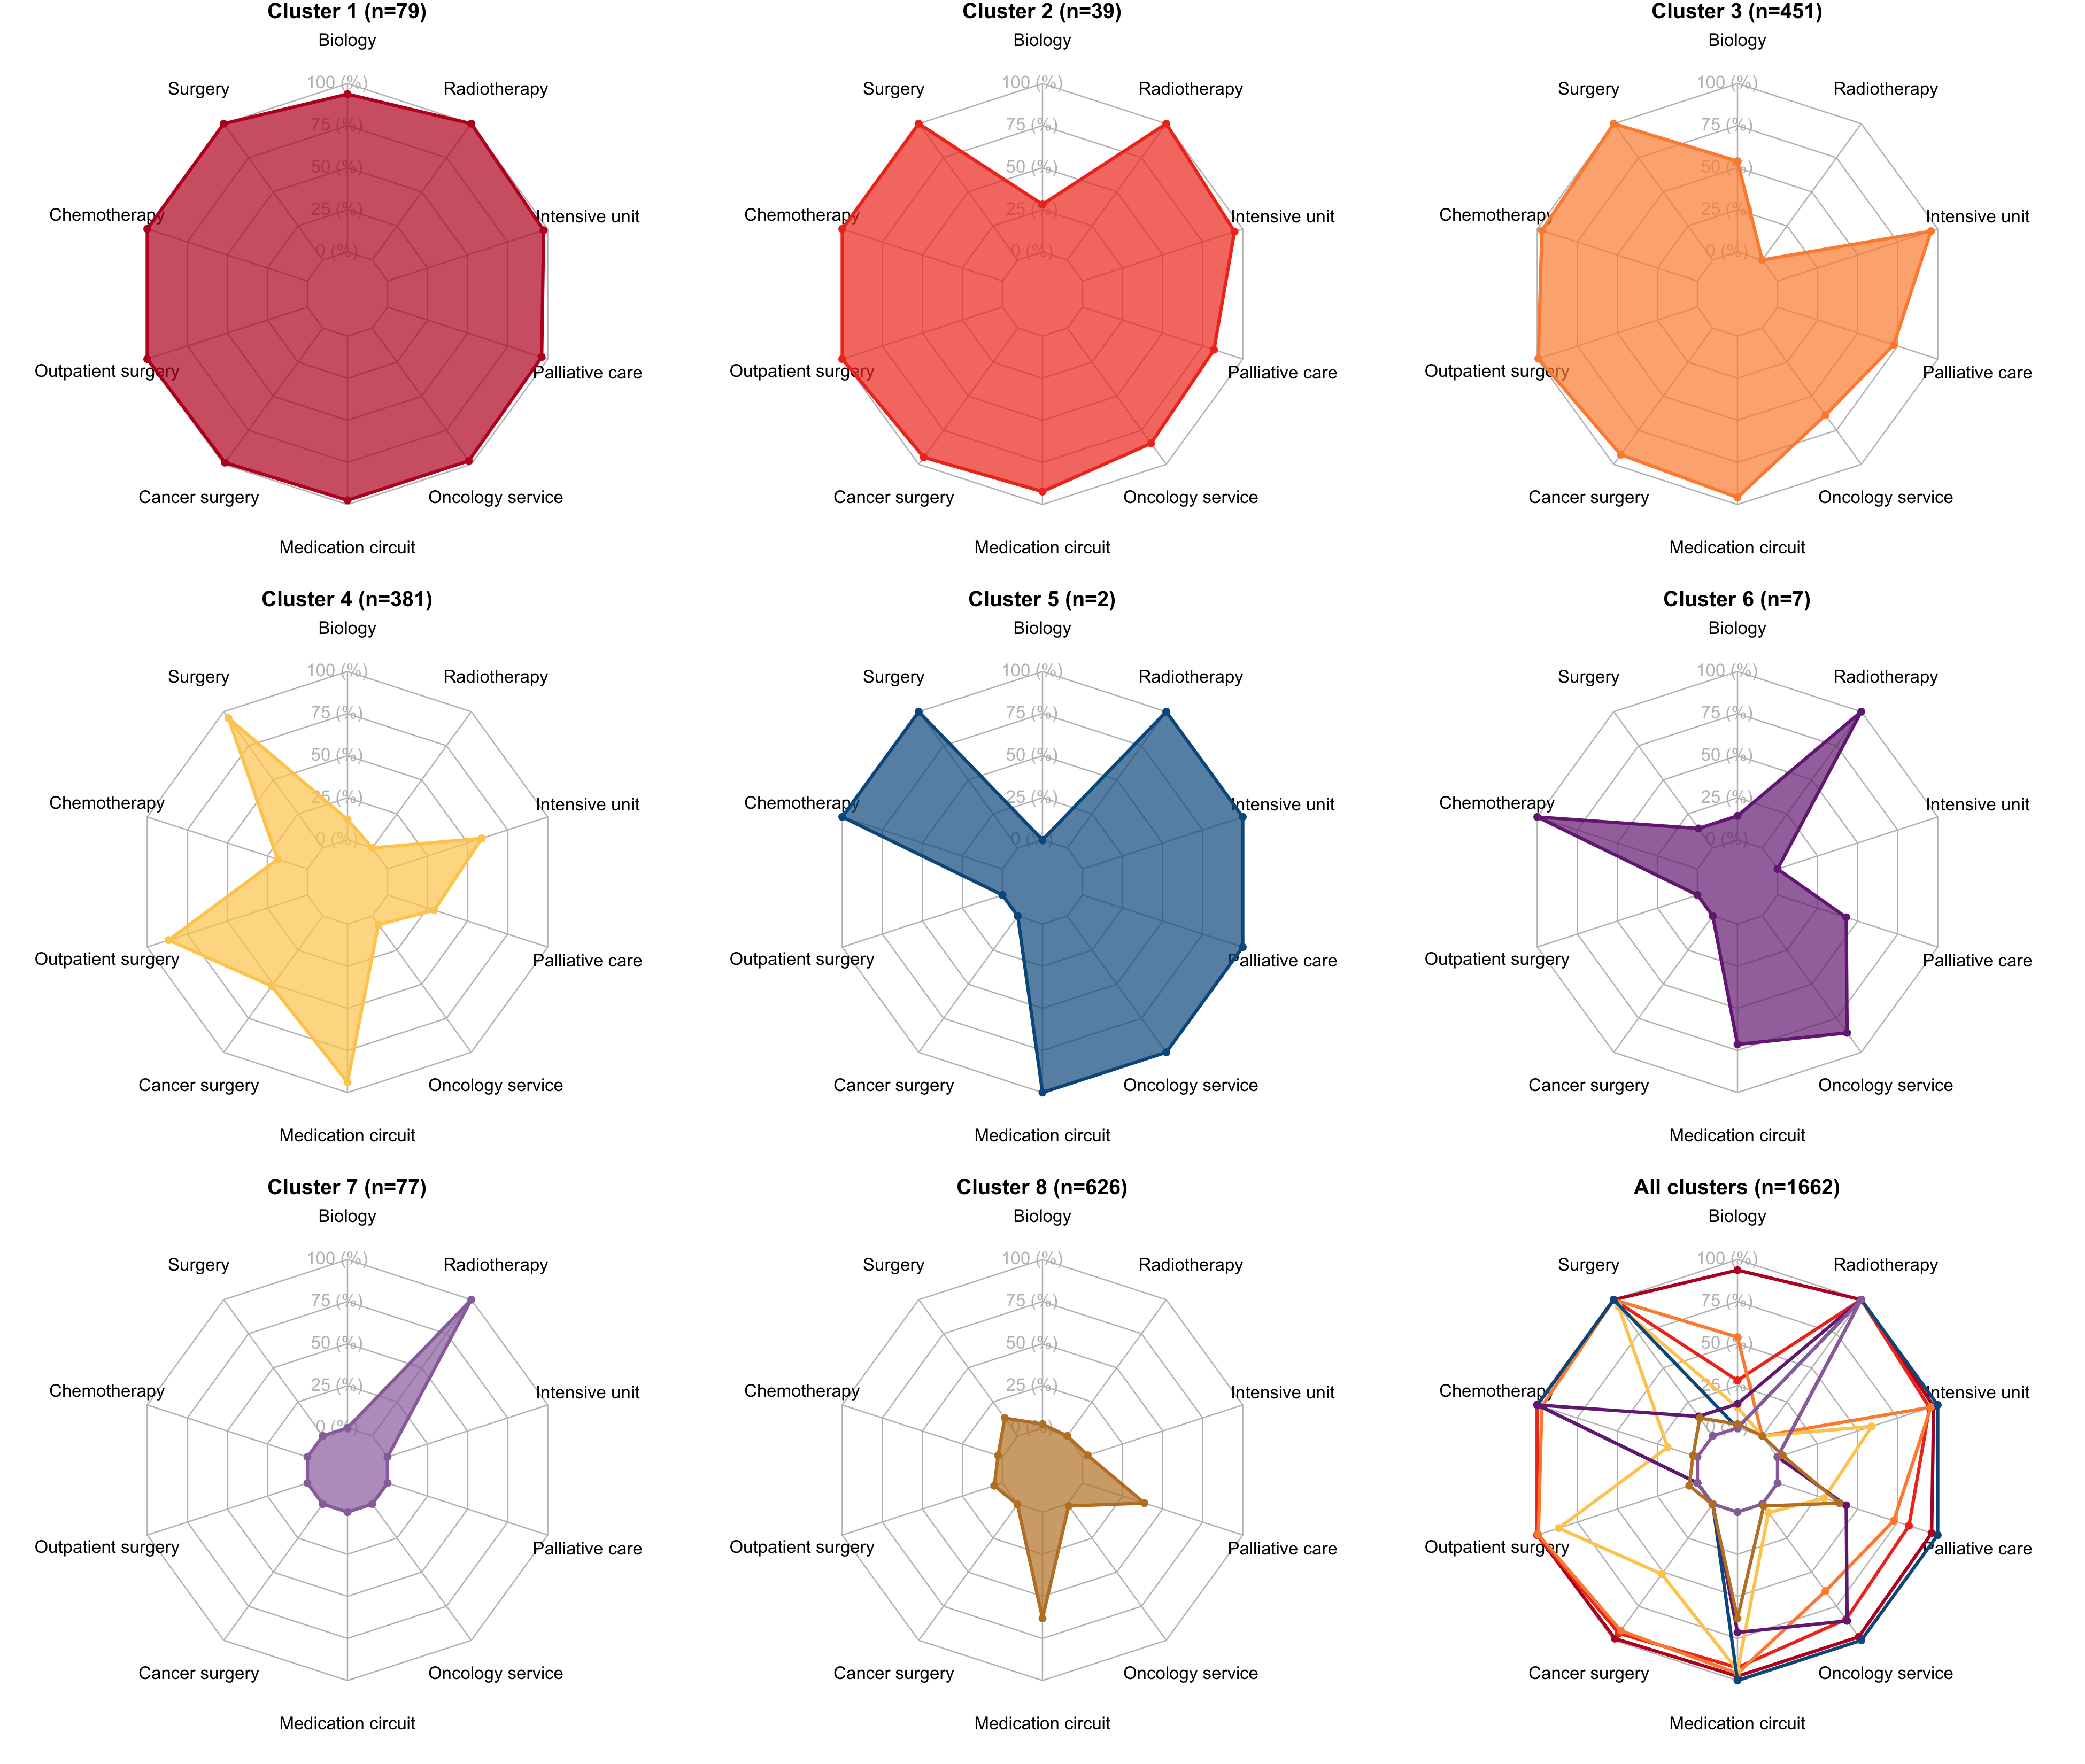
\includegraphics[width=\textwidth]{images/camion/fig1_clusters_services.png}
\centering
\caption{
Distribution of the care centers services and equipment per cluster. Each radar plot axis shows the percentage of the care centers within the cluster that have the corresponding attribute. In Cluster 1, the care centers have all the listed services. In cluster 8, the centers have almost none of the services. Care centers from cluster 1 (n=79) and cluster 2 (n=39) are the most suit-ed for oncology care.
}
\end{figure}